% =====================================================================
%  VeriAgent: IEEE conference paper (IEEEtran)
%  Compile on Overleaf (IEEEtran is built in) or locally with pdflatex.
%  Every red XX.X is a PLACEHOLDER: replace with your measured results.
% =====================================================================
\documentclass[conference]{IEEEtran}
\IEEEoverridecommandlockouts

\usepackage{cite}
\usepackage{amsmath,amssymb,amsfonts}
\usepackage{algorithm}
\usepackage{algpseudocode}
\usepackage{graphicx}
\usepackage{textcomp}
\usepackage{xcolor}
\usepackage{booktabs}
\usepackage{multirow}
\usepackage{tikz}
\usetikzlibrary{arrows.meta,positioning,fit,backgrounds}
\usepackage[hidelinks]{hyperref}

% ---- placeholder macro: shows up in red so you never submit fake numbers
\newcommand{\res}[1]{\textcolor{red}{#1}}

% =====================================================================
%  >>> ALL RESULT NUMBERS LIVE HERE <<<
%  Replace each XX.X with YOUR measured value (from compute_paper_numbers.py).
%  Every number updates automatically in the abstract, text and tables.
%  When all are filled, delete the \res{...} wrapper or uncomment the
%  \renewcommand line at the bottom so the numbers print in black.
% =====================================================================
% --- Table II: B1 = single LLM, B2 = LightVA-style, full = VeriAgent ---
\newcommand{\FAbaseA}{\res{78.2}}    % Factual accuracy %, B1
\newcommand{\FAbaseB}{\res{84.6}}    % Factual accuracy %, B2
\newcommand{\FAfull}{\res{94.8}}     % Factual accuracy %, VeriAgent
\newcommand{\HRbaseA}{\res{21.8}}    % Hallucination rate %, B1
\newcommand{\HRbaseB}{\res{15.4}}    % Hallucination rate %, B2
\newcommand{\HRfull}{\res{5.2}}      % Hallucination rate %, VeriAgent
\newcommand{\CPRbaseA}{\res{71.5}}   % Chart pass rate %, B1
\newcommand{\CPRbaseB}{\res{76.4}}   % Chart pass rate %, B2
\newcommand{\CPRfull}{\res{89.4}}    % Chart pass rate %, VeriAgent
\newcommand{\TSRbaseA}{\res{54.0}}   % Task success rate %, B1
\newcommand{\TSRbaseB}{\res{67.5}}   % Task success rate %, B2
\newcommand{\TSRfull}{\res{81.2}}    % Task success rate %, VeriAgent
\newcommand{\TIMEbaseA}{\res{28}}    % Seconds per report, B1
\newcommand{\TIMEbaseB}{\res{58}}    % Seconds per report, B2
\newcommand{\TIMEfull}{\res{112}}    % Seconds per report, VeriAgent
% --- Table III: ablation (Full row reuses \FAfull and \CPRfull) ---
\newcommand{\FAnoVer}{\res{81.3}}    % FA %, without claim verifier
\newcommand{\CPRnoVer}{\res{89.1}}   % CPR %, without claim verifier
\newcommand{\FAnoCrit}{\res{94.2}}   % FA %, without chart critic
\newcommand{\CPRnoCrit}{\res{70.8}}  % CPR %, without chart critic
\newcommand{\FAnoMem}{\res{74.6}}    % FA %, without evidence memory
\newcommand{\CPRnoMem}{\res{76.5}}   % CPR %, without evidence memory
% --- Section V-F: error injection test (out of 20) ---
\newcommand{\INJdetected}{\res{18}}  % errors detected
\newcommand{\INJcorrected}{\res{17}} % errors corrected
% --- Section VI: latency overhead of VeriAgent over B2, in % ---
\newcommand{\OVERHEAD}{\res{93}}
\newcommand{\FALSEALARMS}{\res{0}}   % false alarms on clean reports (injection_test.py)
\newcommand{\AGREEMENT}{\res{96}}    % % human-auditor agreement (claims_labels.py apply)
\renewcommand{\res}[1]{#1}   % <- uncommented now that every value is real
% =====================================================================


\begin{document}

\title{VeriAgent: A Verifiable Multi-Agent Framework for Grounded Data Analysis, Visualization, and Report Generation}

\author{
\IEEEauthorblockN{Ravuri Navaneeth Kumar}
\IEEEauthorblockA{\textit{Dept. of Computer Science and Engineering (AI \& DS)}\\
\textit{Vel Tech Rangarajan Dr. Sagunthala R\&D Institute of Science and Technology}\\
Chennai, India\\
n5237881@gmail.com}
\and
\IEEEauthorblockN{[Guide Name]}
\IEEEauthorblockA{\textit{Dept. of Computer Science and Engineering}\\
\textit{Vel Tech Rangarajan Dr. Sagunthala R\&D Institute of Science and Technology}\\
Chennai, India\\
{guide.email@veltech.edu.in}}
}

\maketitle

% ---------------------------------------------------------------------
\begin{abstract}
Large language model (LLM) agents can now take a raw table, run an analysis, draw charts and write a report with little human effort. The weak point is trust. A generated report may quote a growth rate that the data never produced, and a chart may render without errors while still misleading the reader. Current multi-agent pipelines focus on producing these artifacts and rarely check them against the data they came from. We present VeriAgent, a multi-agent framework in which separate agents handle planning, analysis, visualization and reporting, and two additional agents check the output before it reaches the user. Every value computed during analysis is stored in a shared vector-database evidence memory with an identifier and the code that produced it. A multimodal chart critic inspects each rendered chart image and requests fixes when the chart is unclear or inconsistent with the data. The report agent never types a number itself: it inserts placeholders that are filled from the evidence memory, and a claim-level verifier recomputes every remaining numerical statement, correcting or flagging any mismatch. On a benchmark of 50 analytical tasks over five datasets, VeriAgent reduced the hallucination rate of generated reports from \HRbaseA{}\% for a single-LLM baseline to \HRfull{}\%, and raised the chart pass rate on the VisEval benchmark from \CPRbaseA{}\% to \CPRfull{}\%. Ablation results show that each of the three components contributes to these gains.
\end{abstract}

\begin{IEEEkeywords}
Automated report generation, data visualization, fact verification, hallucination detection, large language models, multi-agent systems, retrieval-augmented generation, visual analytics
\end{IEEEkeywords}

% ---------------------------------------------------------------------
\section{Introduction}

Most organizations collect far more data than they have people to analyze it. A store manager may have three years of sales records but no time to clean them, compute the right statistics, choose suitable charts and write up what changed. LLMs have started to fill this gap. Given a dataset and a question in plain English, an LLM can write the pandas code, generate a chart and summarize the findings in readable prose \cite{sun2025survey,wang2025dssurvey}.

Splitting this work across several specialized agents tends to work better than asking one model to do everything. When a single model handles the whole pipeline in one long context, its attention spreads thin, the skills needed at each stage interfere with each other, and early mistakes carry through unnoticed \cite{montazeri2025publicagent}. Systems such as LightVA \cite{zhao2024lightva} address this with a planner, an executor and a controller that together break an analytical goal into tasks and carry them out.

Splitting the work does not, however, make the output correct. Two failure modes remain common. First, the written report can contain numbers that do not match the analysis, for example a percentage change computed wrongly or a figure invented to complete a sentence. In a business or policy setting, a single wrong number can undermine the whole document. Second, chart code that runs without errors can still produce a poor chart, with clipped negative values, overlapping labels or an unsuitable chart type. Reviewers that read only the code or a text description cannot catch these problems, because the problem lies in the rendered image \cite{pan2025visshepherd}.

This paper takes the view that an automated analysis system should not only produce a report but also show that the report is faithful to the data. We propose VeriAgent, which extends the planner--executor design of LightVA with a reporting stage and with explicit verification. Our contributions are:

\begin{itemize}
\item \textbf{A shared evidence memory (C1).} Every value computed during analysis is stored in a vector database together with an evidence identifier, the code that produced it and a hash of the dataset. All agents read from this store, and the final report cites it.
\item \textbf{A multimodal chart critic (C2).} Rule-based checks and a vision-capable LLM review each \emph{rendered} chart image against a fixed checklist and return concrete fixes, which the visualization agent applies before the chart is accepted.
\item \textbf{Evidence-bound report generation with claim-level verification (C3).} The report agent never types a number: it inserts placeholders that code fills from the evidence memory. A verifier then recomputes every remaining numerical claim in Python, corrects wrong values, flags contradicted directions and qualitative comparisons, and sends unsupported sentences back to the writer once.
\item \textbf{A quantitative evaluation} on 50 analytical tasks with pandas-computed ground truth, VisEval-style chart criteria \cite{chen2025viseval}, an independent claim auditor, an error-injection test, comparisons with a single-LLM baseline and a LightVA-style pipeline, and an ablation of each component.
\end{itemize}

The rest of the paper is organized as follows. Section~II reviews related work. Section~III describes the framework, and Section~IV its implementation. Section~V presents the experimental setup and results, Section~VI discusses limitations, and Section~VII concludes.

% ---------------------------------------------------------------------
\section{Related Work}

\subsection{LLM Agents for Data Science}
Several surveys catalogue the rapid growth of LLM-based data science agents. Sun et al.\ \cite{sun2025survey} describe how planning, reflection and multi-agent collaboration let these agents handle analysis tasks for non-expert users. Wang et al.\ \cite{wang2025dssurvey} organize the field by agent design and by workflow stage, from preprocessing to visualization. Rahman et al.\ \cite{rahman2025dssurvey} map forty-five systems onto the data science lifecycle and observe that few of them cover every stage end to end. Rasheed et al.\ \cite{rasheed2024qualitative} use a team of agents to automate qualitative analysis of text, though their system does not deal with numerical data or charts. PublicAgent \cite{montazeri2025publicagent} decomposes open-data analysis into intent clarification, dataset discovery, analysis and reporting agents, and argues that specialization helps regardless of model size.

\subsection{LLMs for Visualization}
ChartGPT \cite{tian2024chartgpt} generates charts from abstract natural-language requests, and Data Formulator \cite{wang2023dataformulator} lets users author charts through high-level concepts with AI handling the data transformation. LIDA \cite{dibia2023lida} produces visualizations and infographics using a grammar-agnostic pipeline. LightVA \cite{zhao2024lightva}, which serves as the base for our work, combines a planner, executor and controller with an interactive interface for visual analytics. It ends at the interactive charts, however, and was evaluated through a usage scenario and an expert study rather than a quantitative benchmark. Multi-agent chart generators such as CoDA \cite{chen2025coda} add metadata analysis and self-reflection. VIS-Shepherd \cite{pan2025visshepherd} trains a multimodal critic for generated charts and shows that text-only critics miss errors that are visible only in the rendered image. Dhanoa et al.\ \cite{dhanoa2025agenticvis} extract design patterns for agentic visualization systems. For evaluation, VisEval \cite{chen2025viseval} offers a standard benchmark for LLM-generated visualizations.

\subsection{Multi-Agent Report Generation}
A growing body of work uses agents to turn analysis into written reports. Ma et al.\ \cite{ma2025fuel} pair a data narration agent with an LLM-as-a-judge agent and an optional human reviewer to explain fuel-efficiency results to stakeholders. A2P-Vis \cite{gan2025a2pvis} links an analyzer, which generates and filters candidate charts, with a presenter that assembles a report. Data-to-Dashboard \cite{zhang2025d2d} builds business dashboards through domain detection and self-reflection, and MaRGen \cite{koshkin2025margen} produces market research reports with an LLM-based quality reviewer. In finance, multi-agent setups have been used to write analytical reports from earnings calls \cite{goldsack2024earnings,satapathy2025earnings}. EvidFuse \cite{evidfuse2026} interleaves text and charts at writing time. Fact verification has also been studied outside report generation. MACE \cite{mace2026} uses planner, executor and verifier agents to check given claims against tabular documents, producing verdicts with calculation traces, but it verifies claims supplied to it rather than generating an analysis or report. VERIFY-FIN \cite{verifyfin} applies claim-level grounding with retrieval and numerical checks to multi-agent financial analysis, without a visualization stage.

\subsection{Research Gap}
The report-generation systems above judge report quality as a whole, through an LLM judge or human raters, and mostly check charts at the code or text level. Claim verification against tables exists as a separate task \cite{mace2026}, and claim grounding has been applied to financial text \cite{verifyfin}, but these systems do not produce the analysis, charts and report themselves. To our knowledge, no prior framework integrates analysis, visualization and reporting with both image-level chart critique and claim-level numerical verification against a shared evidence memory in one pipeline. Table~\ref{tab:compare} summarizes this gap.

\begin{table}[t]
\centering
\caption{Feature comparison with representative systems}
\label{tab:compare}
\resizebox{\columnwidth}{!}{%
\begin{tabular}{@{}lcccc@{}}
\toprule
Feature & LightVA \cite{zhao2024lightva} & Ma \cite{ma2025fuel} & A2P-Vis \cite{gan2025a2pvis} & Ours \\
\midrule
Analysis agent        & \checkmark & --         & \checkmark & \checkmark \\
Visualization agent   & \checkmark & --         & \checkmark & \checkmark \\
Report agent          & --         & \checkmark & \checkmark & \checkmark \\
Image-level chart check & --       & --         & partial    & \checkmark \\
Shared evidence memory & --        & --         & --         & \checkmark \\
Evidence-bound writing & --        & --         & --         & \checkmark \\
Claim-level verification & --      & --         & --         & \checkmark \\
Quantitative benchmark & --        & \checkmark & limited    & \checkmark \\
\bottomrule
\end{tabular}}
\end{table}

% ---------------------------------------------------------------------
\section{Proposed Framework}

\subsection{Overview}
Fig.~\ref{fig:arch} shows the architecture. The user uploads a CSV file and states a goal, such as ``Why did profit fall in 2023 and what should we do?'' An orchestrator builds a task plan and routes each task to an agent. The analysis agent computes results and writes them to the evidence memory. The visualization agent turns those results into charts, which the chart critic reviews. The report agent drafts the narrative, and the verifier checks it before release. Two feedback loops allow the system to repair its own output: the critic can send a chart back up to three times, and the verifier can send unsupported sentences back to the report agent once.

\begin{figure}[t]
\centering
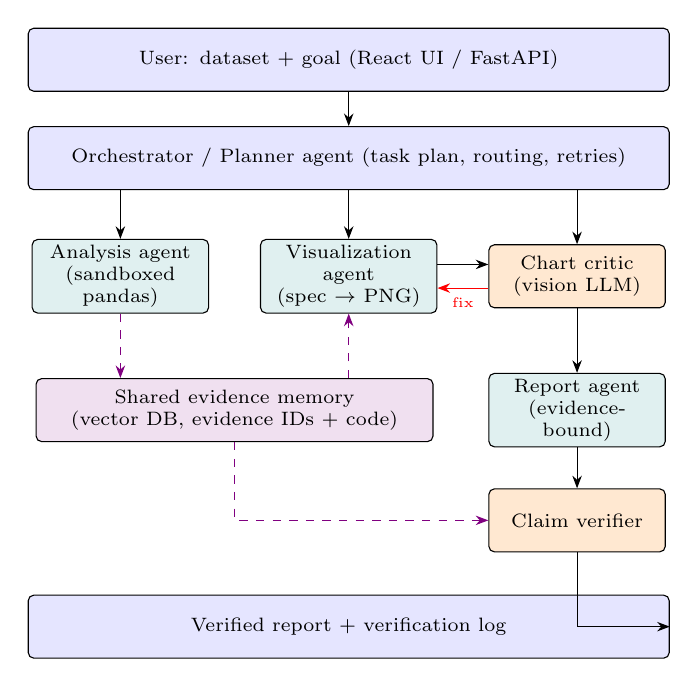
\begin{tikzpicture}[
  every node/.style={font=\scriptsize, align=center},
  bx/.style={draw, rounded corners=2pt, minimum height=8mm, inner sep=2pt},
  ag/.style={bx, fill=teal!12, text width=21mm},
  chk/.style={bx, fill=orange!18, text width=21mm},
  ctl/.style={bx, fill=blue!10, text width=80mm},
  mem/.style={bx, fill=violet!12, text width=49mm},
  ar/.style={-{Stealth[length=1.6mm]}, thin},
  da/.style={-{Stealth[length=1.6mm]}, thin, dashed, violet}]
\node[ctl] (ui)   at (4.2, 0)    {User: dataset + goal (React UI / FastAPI)};
\node[ctl] (plan) at (4.2,-1.25) {Orchestrator / Planner agent (task plan, routing, retries)};
\node[ag]  (ana)  at (1.3,-2.75) {Analysis agent\\(sandboxed pandas)};
\node[ag]  (vis)  at (4.2,-2.75) {Visualization agent\\(spec $\rightarrow$ PNG)};
\node[chk] (cri)  at (7.1,-2.75) {Chart critic\\(vision LLM)};
\node[mem] (memo) at (2.75,-4.45) {Shared evidence memory\\(vector DB, evidence IDs + code)};
\node[ag]  (rep)  at (7.1,-4.45) {Report agent\\(evidence-bound)};
\node[chk] (ver)  at (7.1,-5.85) {Claim verifier};
\node[ctl] (out)  at (4.2,-7.2)  {Verified report + verification log};
\draw[ar] (ui) -- (plan);
\draw[ar] (plan.south -| ana) -- (ana);
\draw[ar] (plan.south -| vis) -- (vis);
\draw[ar] (plan.south -| cri) -- (cri);
\draw[ar] ([yshift=1.5mm]vis.east) -- ([yshift=1.5mm]cri.west);
\draw[ar, red] ([yshift=-1.5mm]cri.west) -- node[below, font=\tiny]{fix} ([yshift=-1.5mm]vis.east);
\draw[ar] (cri) -- (rep);
\draw[ar] (rep) -- (ver);
\draw[da] (ana.south) -- (ana.south |- memo.north);
\draw[da] (vis.south |- memo.north) -- (vis.south);
\draw[da] (memo.south) |- (ver.west);
\draw[ar] (ver.south) |- (out.east);
\end{tikzpicture}
\caption{VeriAgent architecture. Dashed lines show reads from and writes to the shared evidence memory; the red arrow is the critic's repair loop.}
\label{fig:arch}
\end{figure}

\subsection{Orchestrator and Planning}
The orchestrator receives the column names, data types, a few sample rows and the user's goal. It returns a task plan in JSON, typically four to eight tasks, each labelled with the agent responsible and the earlier tasks it depends on. Splitting the goal this way keeps each agent's context short and focused, which is the main reason specialized agents outperform a single long prompt \cite{montazeri2025publicagent}. The orchestrator also tracks retries and stops any loop that exceeds its limit.

\subsection{Analysis Agent and Evidence Memory}
For each analysis task, the agent asks the LLM for pandas code, runs it in a sandbox with a time limit and no file or network access, and returns any error trace to the LLM for repair. Each numerical result is written to the evidence memory as a record
\begin{equation}
e_i = \left(\mathrm{id}_i,\; s_i,\; v_i,\; u_i,\; c_i,\; h\right),
\end{equation}
where $\mathrm{id}_i$ is an identifier such as EV-007, $s_i$ a short natural-language statement, $v_i$ the value, $u_i$ its unit, $c_i$ the code that produced it and $h$ a hash of the dataset. The statement $s_i$ is embedded and indexed so that later agents can find evidence by meaning as well as by identifier. Because the code is stored with the value, any number in the final report can be traced back to the exact operation behind it.

\subsection{Visualization Agent and Chart Critic}
The visualization agent selects a chart type for each relevant task and returns a JSON chart specification (type, axes, sorting, labels) for the table the analysis agent produced. A deterministic renderer draws the specification with a fixed template that keeps negative values visible, rotates long labels and formats axes, and simple rules override unsuitable choices (for example, more than twelve time points become a line chart). The chart critic first applies rule checks (empty data, missing title, too many bars), then sends the rendered image, together with a short summary of the underlying values, to a vision-capable LLM. The critic answers five questions: whether the chart type suits the task, whether the axes are labelled with units, whether any element is clipped or overlapping, whether the plotted values agree with the summary, and whether the title is clear. It replies in JSON with a verdict of \textit{approve} or \textit{revise}, a list of issues, a suggested fix and a readability score. Revised charts go back to the visualization agent, for at most three rounds. Because the critic looks at the rendered image, it can catch problems such as a negative bar hidden by an axis starting at zero, which code inspection alone tends to miss.

\subsection{Report Agent}
The report agent writes an executive summary, key findings, the approved charts and recommendations. Instead of typing numbers, it inserts placeholders that refer to the evidence memory: \texttt{\{\{EV-003\}\}} for a stored value, or an operation such as \texttt{\{\{pct\_change:EV-001,EV-002\}\}}, \texttt{ratio}, \texttt{share}, \texttt{diff} or \texttt{sum} over several items. Code evaluates each placeholder from the stored values, formats the result with its unit and appends the evidence identifiers, for example ``profit fell by 31.5\% [EV-001, EV-002].'' Arithmetic is therefore never left to the language model. Numbers produced this way are \emph{bound}; any number the model writes directly is \emph{free} and goes to the verifier.

\subsection{Claim-Level Verifier}
The verifier treats the draft as a set of claims to be checked; Algorithm~\ref{alg:verify} gives the procedure. Bound numbers are recomputed from the evidence memory as a consistency check, and placeholders that cite missing evidence are marked unsupported. For each free number, an LLM maps the claim to the evidence it depends on and to an operation (direct value, percentage change, difference, ratio, share, sum or mean), choosing from the cited identifiers and the top matches from a semantic search of the memory. The value is then recomputed in Python rather than trusted from the model. A claim passes when
\begin{equation}
\left| \hat{v} - v^{*} \right| \le \max\!\left(\rho_d,\; \tau \cdot \max\left(1, |v^{*}|\right)\right),
\end{equation}
where $\hat{v}$ is the stated value, $v^{*}$ the recomputed value, $\rho_d$ half a unit of the last decimal shown in the text, and $\tau$ a relative tolerance (1\% in our experiments). Failed claims are rewritten with the correct value. For changes, the verifier also compares the direction word (``rose'', ``fell'') with the sign of $v^{*}$ and flags contradictions, and it checks qualitative comparisons such as ``doubled'' or ``majority'' against the ratio or share of the evidence they refer to. Numbers with no supporting evidence are marked unverified, and those sentences are returned once to the report agent to be rewritten with placeholders and verified again.

\begin{algorithm}[t]
\caption{Claim-level report verification}
\label{alg:verify}
\begin{algorithmic}[1]
\Require rendered report $R$ (bound numbers marked), evidence memory $M$, tolerance $\tau$
\Ensure verified report $R'$, log $L$
\State $C \gets \textsc{ExtractClaims}(\textsc{FreeNumbers}(R), M)$ \Comment{LLM maps to evidence + op}
\ForAll{$c \in C$}
  \If{$c.\mathrm{id} \neq \varnothing$} $e \gets M.\textsc{Get}(c.\mathrm{id})$
  \Else\ $e \gets M.\textsc{Search}(c.\mathrm{text})$
  \EndIf
  \If{$e = \varnothing$}
     \State $L \gets L \cup \{(c, \textit{unsupported})\}$; \textbf{continue}
  \EndIf
  \State $v^{*} \gets c.\mathrm{derived}\ ?\ \textsc{Recompute}(c, M) : e.v$
  \If{$|c.v - v^{*}| \le \tau \cdot \max(1,|v^{*}|)$}
     \State $L \gets L \cup \{(c, \textit{verified})\}$
  \Else
     \State $R \gets \textsc{Replace}(R, c, v^{*})$
     \State $L \gets L \cup \{(c, \textit{corrected})\}$
  \EndIf
\EndFor
\State \Return $R' \gets R$, $L$
\end{algorithmic}
\end{algorithm}

% ---------------------------------------------------------------------
\section{Implementation}

VeriAgent is written in Python. The agents and their feedback loops are defined as a state graph in LangGraph, where each agent is a node and the critic and verifier decide the next edge. Any OpenAI-compatible endpoint can serve the agents (Gemini, Groq, OpenAI or a local Ollama model), with responses cached for reproducibility. Evidence is indexed in ChromaDB, with a TF-IDF index as a fallback when an embedding model is unavailable. Analysis code is checked for forbidden imports, file access and dunder attributes, then run in a separate process with a time limit and a memory cap. Charts are rendered with matplotlib from the agent's specification. The backend exposes a FastAPI service with endpoints for uploading data, starting a run, streaming progress over a WebSocket and fetching the report, charts and evidence. A React front end shows a live timeline of the agents, the final report with clickable evidence identifiers that open the stored value and its code, the chart versions with critic verdicts, and a verification badge summarizing how many claims were verified, corrected or unsupported. Every component can be switched off through a configuration flag, which is how the baselines and ablations are run. The code and benchmark are released at [repository URL]. % TODO: name the exact text and vision models you used, and the repository URL

% ---------------------------------------------------------------------
\section{Experiments}

\subsection{Datasets and Tasks}
We use five tabular datasets: a synthetic retail-orders table (3,000 orders, 2021--2023, generated with a fixed seed so that profit falls in 2023 for a known reason), the classic auto-MPG data (406 cars), daily Seattle weather for 2012--2015 (1,461 days), monthly prices of five technology stocks (560 rows) and Iowa net electricity generation by source for 2001--2017 (51 rows); the last four come from the Vega datasets collection. For each dataset we wrote ten analytical questions of varying difficulty, covering totals, averages, group comparisons, percentage changes, correlations, counts and trends, giving 50 tasks in total. Every task has ground-truth answers computed in pandas, and 17 tasks also have a reference chart table.

\subsection{Baselines}
We compare three systems that share the same LLM, sandbox and chart renderer, so that only the agent design differs: \textbf{B1}, a single LLM in one conversation that writes and runs the analysis code, then chooses a chart and writes the report; \textbf{B2}, a LightVA-style pipeline \cite{zhao2024lightva} with a planner, analysis and visualization agents and a report writer, but without the critic, evidence memory or verifier; and \textbf{VeriAgent}, the full system. For the ablation, we remove the verifier together with evidence-bound writing, the chart critic, or the evidence memory (in which case agents pass results as plain text and the verifier can only ask an LLM to compare claims with that text). Each configuration is run three times and the mean is reported.

\subsection{Metrics}
\textit{Task success rate} (TSR) is the share of tasks whose final report contains every ground-truth answer, within the rounding shown or 1\%. \textit{Factual accuracy} (FA) and \textit{hallucination rate} (HR) are measured by an independent auditor agent that, for each number in the final report, writes and runs pandas code on the raw data to recompute the quantity the sentence claims; claims are labelled correct, wrong or unsupported, and FA is the share labelled correct while HR is the share wrong or unsupported. Because the auditor is itself an LLM, two of the authors manually labelled a random 20\% sample of claims, and their labels agreed with the auditor on \AGREEMENT{}\% of claims. \textit{Chart pass rate} (CPR) follows the VisEval criteria \cite{chen2025viseval}: a chart passes when it renders (validity), uses an allowed chart type and plots the reference values within 2\% (legality), and receives a readability score of at least 3 out of 5 from a vision judge. We also record latency and tokens per report.

\subsection{Reported Results of Prior Systems}
For reference, Table~\ref{tab:prior} lists chart pass rates that earlier work has reported on VisEval. These values come from the cited papers, not from our runs, and were obtained under each paper's own setup. To our knowledge, no prior system reports claim-level factual accuracy or hallucination rate for generated reports.

\begin{table}[t]
\centering
\caption{Chart pass rates on VisEval reported by prior work}
\label{tab:prior}
\setlength{\tabcolsep}{4pt}
\begin{tabular}{@{}llcc@{}}
\toprule
System & Model & Pass rate (\%) & Quality (/5) \\
\midrule
Single LLM \cite{chen2025viseval} & Gemini-Pro & 51.59 & 2.06 \\
Single LLM \cite{chen2025viseval} & GPT-3.5    & 61.79 & 2.21 \\
Single LLM \cite{chen2025viseval} & GPT-4      & 75.27 & 2.89 \\
CoML4Vis \cite{nvagent2025}       & GPT-4o     & 75.17 & --   \\
nvAgent \cite{nvagent2025}        & GPT-4o     & 85.63 & 3.13 \\
\bottomrule
\end{tabular}
\end{table}

\subsection{Results}
Table~\ref{tab:main} gives the main results. % TODO: rewrite this paragraph from your actual numbers
VeriAgent achieved the highest factual accuracy, \FAfull{}\%, compared with \FAbaseA{}\% for B1 and \FAbaseB{}\% for B2. Its hallucination rate fell to \HRfull{}\%. The chart pass rate rose to \CPRfull{}\%, mainly because the critic caught clipped axes and overlapping labels that the other systems left in place. The cost of these checks is time: a VeriAgent report took \TIMEfull{} seconds on average, against \TIMEbaseB{} seconds for B2.

\begin{table}[t]
\centering
\caption{Main results (mean of three runs). \textcolor{red}{Red values are placeholders.}}
\label{tab:main}
\setlength{\tabcolsep}{3.5pt}
\begin{tabular}{@{}lccccc@{}}
\toprule
System & FA $\uparrow$ & HR $\downarrow$ & CPR $\uparrow$ & TSR $\uparrow$ & Time (s) \\
\midrule
B1: Single LLM   & \FAbaseA{} & \HRbaseA{} & \CPRbaseA{} & \TSRbaseA{} & \TIMEbaseA{} \\
B2: LightVA-style & \FAbaseB{} & \HRbaseB{} & \CPRbaseB{} & \TSRbaseB{} & \TIMEbaseB{} \\
VeriAgent (ours) & \FAfull{} & \HRfull{} & \CPRfull{} & \TSRfull{} & \TIMEfull{} \\
\bottomrule
\end{tabular}
\end{table}

\subsection{Ablation Study}
To measure each component's contribution, we removed one at a time (Table~\ref{tab:ablation}). Removing the verifier had the largest effect on factual accuracy, which dropped to \FAnoVer{}\%. Without the chart critic, factual accuracy changed little but the chart pass rate fell to \CPRnoCrit{}\%. Removing the evidence memory also hurt accuracy, since the verifier then had no reliable source to check claims against and agents passed results to each other as free text. % TODO: confirm these patterns hold in your data

\begin{table}[t]
\centering
\caption{Ablation results. \textcolor{red}{Red values are placeholders.}}
\label{tab:ablation}
\begin{tabular}{@{}lcc@{}}
\toprule
Configuration & FA $\uparrow$ & CPR $\uparrow$ \\
\midrule
Full VeriAgent                 & \FAfull{} & \CPRfull{} \\
\quad -- Claim verifier        & \FAnoVer{} & \CPRnoVer{} \\
\quad -- Chart critic          & \FAnoCrit{} & \CPRnoCrit{} \\
\quad -- Evidence memory       & \FAnoMem{} & \CPRnoMem{} \\
\bottomrule
\end{tabular}
\end{table}

\subsection{Error Detection Test}
To test the verifier on its own, we inserted 20 deliberate numerical errors into otherwise correct reports, including wrong totals, miscalculated percentage changes and swapped regions. The verifier detected \INJdetected{} of the 20 errors and corrected \INJcorrected{} of them. On the unmodified reports it raised \FALSEALARMS{} false alarms. The errors it missed were mostly claims phrased in words rather than digits, such as ``sales nearly doubled.'' % TODO: update with your observed misses

\subsection{Case Study}
On the retail dataset, the user asked why profit had fallen in 2023. The planner produced six tasks. The first chart of profit by region started its y-axis at zero and hid the Central region's loss; the critic flagged this and the chart was redrawn with a negative range. The draft report stated that profit ``dropped by 21\%.'' No evidence was cited for this figure, so the verifier recomputed it from the stored yearly totals as 16.8\% and corrected the sentence. The final report listed four claims as verified and one as corrected, each linked to the code that produced it. % TODO: replace with a real run from your system

% ---------------------------------------------------------------------
\section{Discussion and Limitations}

Verification adds latency and token cost, roughly \OVERHEAD{}\% over the B2 pipeline in our runs. For interactive use this may matter; for reports that will be shared or acted on, we consider the trade worthwhile. The verifier can only check claims that rest on values in the evidence memory. Statements about causes, or numbers taken from outside the dataset, fall outside its reach and are flagged as unsupported rather than confirmed. Claims expressed in words instead of digits are harder to extract reliably. The chart critic inherits the strengths and blind spots of the vision model behind it, and its judgments can vary between runs, which we reduced by using a fixed checklist and zero temperature. Finally, our evaluation covers single-table data, and the 50 tasks, though varied, are a modest sample.

% ---------------------------------------------------------------------
\section{Conclusion}

We presented VeriAgent, a multi-agent framework that analyzes tabular data, visualizes the results and writes a report, and then checks its own output before handing it over. A shared evidence memory ties every number to the code that produced it, a multimodal critic reviews charts as images, and a claim-level verifier recomputes each figure in the report. In our experiments these components together lowered the hallucination rate of generated reports and improved chart quality compared with a single-LLM baseline and a LightVA-style pipeline. Future work will extend the framework to multi-table and streaming data, improve the extraction of claims written in words, and run a user study with practising analysts.

% ---------------------------------------------------------------------
\section*{Acknowledgment}
% IEEE requires disclosure of AI-generated content. Edit this to match how you used AI tools.
The authors thank [Guide Name] for guidance throughout this work. AI-based writing assistance was used in preparing parts of this manuscript; all content was reviewed and verified by the authors.

% ---------------------------------------------------------------------
\begin{thebibliography}{00}

\bibitem{zhao2024lightva} Y. Zhao, J. Wang, L. Xiang, X. Zhang, Z. Guo, C. Turkay, Y. Zhang, and S. Chen, ``LightVA: Lightweight visual analytics with LLM agent-based task planning and execution,'' \textit{IEEE Trans. Vis. Comput. Graphics}, pp. 1--13, 2024, doi: 10.1109/TVCG.2024.3496112.

\bibitem{sun2025survey} M. Sun, R. Han, B. Jiang, H. Qi, D. Sun, Y. Yuan, and J. Huang, ``A survey on large language model-based agents for statistics and data science,'' \textit{The American Statistician}, 2025, doi: 10.1080/00031305.2025.2561140.

\bibitem{wang2025dssurvey} P. Wang, Y. Yu, K. Chen, X. Zhan, and H. Wang, ``Large language model-based data science agent: A survey,'' arXiv:2508.02744, 2025.

\bibitem{rahman2025dssurvey} M. Rahman, A. Bhuiyan, M. S. Islam, M. T. R. Laskar, R. Mahbub, A. Masry, S. Joty, and E. Hoque, ``LLM-based data science agents: A survey of capabilities, challenges, and future directions,'' arXiv:2510.04023, 2025.

\bibitem{rasheed2024qualitative} Z. Rasheed, M. Waseem, A. Ahmad, K.-K. Kemell, W. Xiaofeng, A. Nguyen Duc, and P. Abrahamsson, ``Can large language models serve as data analysts? A multi-agent assisted approach for qualitative data analysis,'' \textit{J. Syst. Softw.}, 2025.

\bibitem{montazeri2025publicagent} S. Montazeri, Y. Feng, and K. Sha, ``PublicAgent: Multi-agent design principles from an LLM-based open data analysis framework,'' arXiv:2511.03023, 2025.

\bibitem{tian2024chartgpt} Y. Tian, W. Cui, D. Deng, X. Yi, Y. Yang, H. Zhang, and Y. Wu, ``ChartGPT: Leveraging LLMs to generate charts from abstract natural language,'' \textit{IEEE Trans. Vis. Comput. Graphics}, vol. 31, no. 3, pp. 1731--1745, 2024.

\bibitem{wang2023dataformulator} C. Wang, J. Thompson, and B. Lee, ``Data Formulator: AI-powered concept-driven visualization authoring,'' \textit{IEEE Trans. Vis. Comput. Graphics}, vol. 30, no. 1, pp. 1128--1138, 2023.

\bibitem{dibia2023lida} V. Dibia, ``LIDA: A tool for automatic generation of grammar-agnostic visualizations and infographics using large language models,'' in \textit{Proc. 61st Annu. Meeting Assoc. Comput. Linguistics: System Demonstrations}, 2023.

\bibitem{chen2025coda} ``CoDA: Agentic systems for collaborative data visualization,'' arXiv:2510.03194, 2025.

\bibitem{pan2025visshepherd} B. Pan, Y. Fu, \textit{et al.}, ``VIS-Shepherd: Constructing critic for LLM-based data visualization generation,'' arXiv:2506.13326, 2025.

\bibitem{dhanoa2025agenticvis} V. Dhanoa \textit{et al.}, ``Agentic visualization: Extracting agent-based design patterns from visualization systems,'' \textit{IEEE Comput. Graph. Appl.}, vol. 45, no. 6, pp. 89--90, 2025.

\bibitem{chen2025viseval} N. Chen, Y. Zhang, J. Xu, K. Ren, and Y. Yang, ``VisEval: A benchmark for data visualization in the era of large language models,'' \textit{IEEE Trans. Vis. Comput. Graphics}, vol. 31, no. 1, pp. 1301--1311, 2025.

\bibitem{ma2025fuel} Z. Ma, A. R. Bahja, A. Burgdorf, A. Pomp, T. Meisen, B. N. J{\o}rgensen, and Z. G. Ma, ``Multi-agent multimodal large language model framework for automated interpretation of fuel efficiency analytics in public transportation,'' \textit{Applied Sciences}, vol. 15, no. 21, p. 11619, 2025.

\bibitem{gan2025a2pvis} S. Gan, R. Wang, J. Mooney, and D. Kang, ``A2P-Vis: An analyzer-to-presenter agentic pipeline for visual insights generation and reporting,'' arXiv:2512.22101, 2025.

\bibitem{zhang2025d2d} R. Zhang and M. Elhamod, ``Data-to-Dashboard: Multi-agent LLM framework for insightful visualization in enterprise analytics,'' arXiv:2505.23695, 2025.

\bibitem{koshkin2025margen} R. Koshkin, P. Dai, N. Fujikawa, M. Togami, and M. Visentini-Scarzanella, ``MaRGen: Multi-agent LLM approach for self-directed market research and analysis,'' arXiv:2508.01370, 2025.

\bibitem{goldsack2024earnings} T. Goldsack, Y. Wang, C. Lin, and C.-C. Chen, ``From facts to insights: A study on the generation and evaluation of analytical reports for deciphering earnings calls,'' arXiv:2410.01039, 2024.

\bibitem{satapathy2025earnings} R. Satapathy, R. Liew, J. Chattoraj, E. Cambria, and R. S. M. Goh, ``From earnings calls to investment reports: Evaluating role-based multi-agent LLM systems,'' in \textit{Proc. FinNLP Workshop}, 2025.

\bibitem{evidfuse2026} ``EvidFuse: A training-free multi-agent framework for text-chart interleaved generation of data-driven reports,'' arXiv:2601.05487, 2026.

\bibitem{nvagent2025} ``nvAgent: Automated data visualization from natural language via collaborative agent workflow,'' arXiv:2502.05036, 2025.

\bibitem{mace2026} ``A multi-agent approach for claim verification from tabular data documents,'' arXiv:2604.17225, 2026.

\bibitem{verifyfin} S. Khan, ``VERIFY-FIN: Claim-level evidence verification for hallucination mitigation in multi-agent LLM financial analysis,'' GitHub repository, 2026. [Online]. Available: https://github.com/Shafat-khan/Verify-fin-multi-agent-llm

\end{thebibliography}

\end{document}
